\documentclass[border=3pt]{standalone}
% Preâmbulo compartilhado pelos diagramas TikZ da aula
\usepackage[T1]{fontenc}
\usepackage[utf8]{inputenc}
\usepackage{lmodern}
\usepackage{amsmath}
\usepackage{xcolor}
\usepackage{tikz}
\usetikzlibrary{arrows.meta,angles,quotes,decorations.pathmorphing,calc,
                positioning,shapes.geometric,backgrounds,fit}

% Paleta (mesma dos SVGs originais)
\definecolor{dblue}{HTML}{2A5B8C}
\definecolor{dorange}{HTML}{B3541E}
\definecolor{dgreen}{HTML}{4A7C59}
\definecolor{dred}{HTML}{9C4B4B}
\definecolor{dcream}{HTML}{F4F1EA}
\definecolor{dshade}{HTML}{DDD7C9}

% Estilos comuns (prefixo d... para não colidir com chaves internas do pgf)
\tikzset{
  >={Stealth[length=2mm]},
  dguide/.style={gray!55, dashed, line width=0.4pt},
  daxis/.style={gray!60, line width=0.7pt, ->},
  dbody/.style={fill=black!3, draw=black!80, line width=1pt},
  dacc/.style={draw=dblue, line width=1pt},
  dlbl/.style={black!55, font=\small},
  dsub/.style={black!45, font=\footnotesize},
  dstate/.style={circle, draw=black!80, fill=dcream, line width=1pt,
                 minimum size=17mm, font=\large, inner sep=1pt},
  dobs/.style={circle, draw=black!80, fill=dshade, line width=1pt,
               minimum size=14mm, font=\large, inner sep=1pt},
  dbox/.style={rounded corners=2pt, draw=black!80, fill=dcream, line width=1pt,
               align=center, inner sep=6pt},
  dtrans/.style={->, dblue, line width=1pt},
  dmeas/.style={->, dorange, line width=1pt},
}

\begin{document}
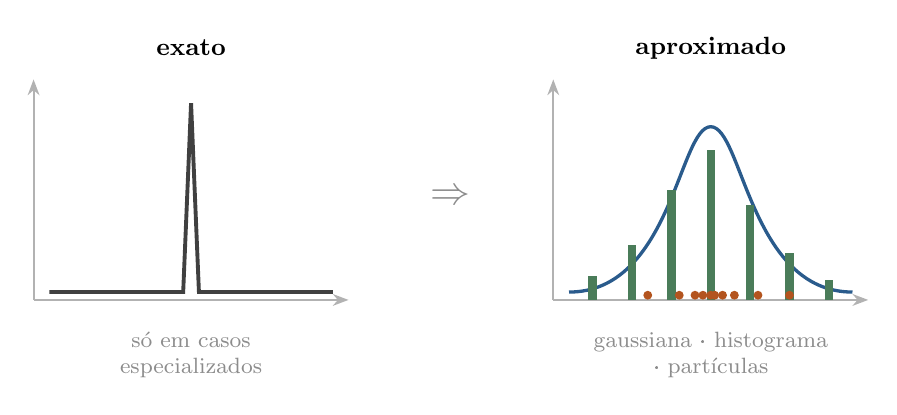
\begin{tikzpicture}[x=1cm,y=1cm]

  % --- exato ---
  \begin{scope}
    \node[font=\small\bfseries] at (2,3.2) {exato};
    \draw[daxis] (0,0) -- (4,0);
    \draw[daxis] (0,0) -- (0,2.8);
    \draw[black!75, line width=1.4pt]
      (0.2,0.1) -- (1.9,0.1) -- (2.0,2.5) -- (2.1,0.1) -- (3.8,0.1);
    \node[dsub, align=center] at (2,-0.7) {só em casos\\especializados};
  \end{scope}

  \node[black!45, font=\Large] at (5.3,1.3) {$\Rightarrow$};

  % --- aproximado ---
  \begin{scope}[shift={(6.6,0)}]
    \node[font=\small\bfseries] at (2,3.2) {aproximado};
    \draw[daxis] (0,0) -- (4,0);
    \draw[daxis] (0,0) -- (0,2.8);
    % gaussiana
    \draw[dblue, line width=1.2pt]
      (0.2,0.1) .. controls (1.5,0.1) and (1.6,2.2) .. (2.0,2.2)
                .. controls (2.4,2.2) and (2.5,0.1) .. (3.8,0.1);
    % histograma
    \foreach \x/\h in {0.5/0.3,1.0/0.7,1.5/1.4,2.0/1.9,2.5/1.2,3.0/0.6,3.5/0.25}
      \draw[dgreen, line width=3pt] (\x,0) -- (\x,\h);
    % partículas
    \foreach \x in {1.2,1.6,1.8,1.9,2.0,2.05,2.15,2.3,2.6,3.0}
      \fill[dorange] (\x,0.06) circle (1.6pt);
    \node[dsub, align=center] at (2,-0.7) {gaussiana · histograma\\· partículas};
  \end{scope}

\end{tikzpicture}
\end{document}
